\setcounter{chapter}{3}
\chapter{视频流Hash}

\section{实验目的}
练习抗碰撞哈希函数的使用,理解哈希函数抗碰撞的安全性。

\section{实验要求}

(前略)...网站不计算整个文件的哈希值,而是将文件分成 1KB 的数据块
(1024 字节)。它计算最后一个块的哈希并将值
附加到倒数第二个块。然后它计算这个增强的倒数第二个块的散列,并将得到
的散列附加到最后的第三个块。此过程从最后一个块继续到第一个块,如下图
所示:

\begin{figure}[!htbp]
\centering
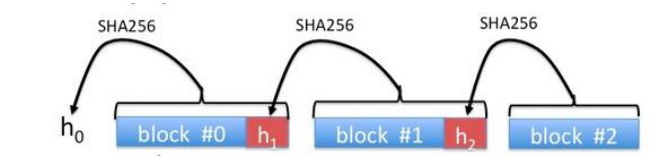
\includegraphics[width=0.8\textwidth]{hash.png}
\end{figure}

网站将最终的哈希值$h_0$通过认证信道分发给用户。

在用户端,浏览器每次下载文件$F$的一个数据块,以及上述所示的附加哈希
值,并进行验证,若验证通过则播放第一个视频块。具体的,通过验证
$H(B_0||h_1)$与$h_0$是否相等来验证第一个区块的完整性; 
通过验证$H(B_1||h_2)$与$h_1$
是否相等来验证第二个区块的完整性;以此类推直至最后一个区块。这样,每
个块都会在收到时进行验证和播放,无需等到整个文件下载完毕。容易证明,
只要哈希函数满足抗碰撞性质,那么攻击者的篡改行为无法通过上述完整性验
证。

本次实验使用 SHA-256 作为哈希函数,实现上述视频验证程序。每一个
哈希值以二进制数据的形式和视频数据块进行链接。若视频数据大小不是 1KB
的整倍数,那么最后一个区块可以小于 1KB,其余的数据区块则需要刚好是
1KB 的整倍数。

程序能够根据输入的文件 $F$计算得到相应的$h_0$,以验证收到文件的正确
性。具体的,请在实验报告中给出视频 1 的$h_0$值(使用 hex 编码)。

\newpage
\section{实验内容}

本实验通过Python语言编写脚本进行,下面具体说明。

\subsection{文件读取}

实验中给到的文件为视频格式,可通过Python语言os库分块读取。

笔者设计了get\_file\_block函数用于进行读取,代码如下:

\begin{lstlisting}[language = Python]
def get_file_block(file_name):
    with open(file_name, 'rb') as f:
        for idx in reversed(range(0, os.path.getsize(file_name), BLOCK_SIZE)):
            f.seek(idx)
            yield f.read(BLOCK_SIZE)
\end{lstlisting}

其中BLOCK\_SIZE为全局变量,定义为1024,通过该函数即可以1 KB的大小,分块读取视频文件。

值得一提的是,笔者使用yield语法进行结果返回,使得函数成为生成器(Generator),可模拟
视频流在实际环境中分块送达的特点。

\subsection{分块哈希}

该部分使用了Crypto库中的SHA256算法,具体代码如下:

\begin{lstlisting}[language = Python]
def stream_hash(file_name):
    hash_result = b''
    for block in get_file_block(file_name):
        h = SHA256.new(block + hash_result) ## Note:1
        hash_result = h.digest()
    return h.hexdigest()
\end{lstlisting}

可注意在Note:1所在行,我们对每块内容加上上一块的哈希值,作为哈希函数的输入,进行计算。

最后返回的哈希值为视频文件的哈希值的hex编码形式。

\section{实验结果}

对于验证性视频6.2.birthday.mp4,得到的哈希值与所给测试结果相同,为:
\begin{center}
    03c08f4ee0b576fe319338139c045c89c3e8e9409633bea29442e21425006ea8
\end{center}

并计算视频6.1.intro.mp4,得到的哈希值为:
\begin{center}
    5b96aece304a1422224f9a41b228416028f9ba26b0d1058f400200f06a589949
\end{center}